\documentclass[final,3p,times,twocolumn]{elsarticle}

%% Use the option review to obtain double line spacing
%% \documentclass[preprint,review,12pt]{elsarticle}

%% Use the options 1p,twocolumn; 3p; 3p,twocolumn; 5p; or 5p,twocolumn
%% for a journal layout:
%% \documentclass[final,1p,times]{elsarticle}
%% \documentclass[final,1p,times,twocolumn]{elsarticle}
%% \documentclass[final,3p,times]{elsarticle}
%% \documentclass[final,3p,times,twocolumn]{elsarticle}
%% \documentclass[final,5p,times]{elsarticle}
%% \documentclass[final,5p,times,twocolumn]{elsarticle}

%% if you use PostScript figures in your article
%% use the graphics package for simple commands
%% \usepackage{graphics}
%% or use the graphicx package for more complicated commands
%% \usepackage{graphicx}
%% or use the epsfig package if you prefer to use the old commands
%% \usepackage{epsfig}

%% The amssymb package provides various useful mathematical symbols
\usepackage{amssymb}
%% The amsthm package provides extended theorem environments
%% \usepackage{amsthm}
%% The bm package lets you access bold symbols in math mode using the \boldsymbol command (useful to get bold greek letters).
\usepackage{bm}
%% The bbm (and also dsfont) package is contains the indicator function symbol \mathbbm{1}
\usepackage{bbm}
\usepackage{dsfont}
%% The amsmath package contains the split environment, letting you split equations into multiple lines.
%% See "https://www.sharelatex.com/learn/Aligning_equations_with_amsmath " for an explanation.
\usepackage{amsmath}
%% The lineno packages adds line numbers. Start line numbering with
%% \begin{linenumbers}, end it with \end{linenumbers}. Or switch it on
%% for the whole article with \linenumbers after \end{frontmatter}.
%% \usepackage{lineno}
%% The algorithm package defines the algorithm floating environment and the algpseudocode package is useful for constructing Pseudo code.
\usepackage{algorithm}
\usepackage{algpseudocode}
%% For making algorithms float
\usepackage{float}
\newfloat{algorithm}{t}{lop}
%% For drawing pictures inside latex
\usepackage{tikz}
%% For setting the 'DRAFT' watermark
%\usepackage{draftwatermark}
%\SetWatermarkText{DRAFT}
%\SetWatermarkScale{1}

%% Declaring \argmin and \argmax operators:
\DeclareMathOperator*{\argmin}{arg\,min}
\DeclareMathOperator*{\argmax}{arg\,max}
%% Declare trace operator \Tr:
\DeclareMathOperator*{\Tr}{Tr}
%% Declare pdf functions
\DeclareMathOperator*{\Dir}{Dir}
\DeclareMathOperator*{\Cat}{Cat}
%% shorthand for \boldsymbol and \overline
\let\bs\boldsymbol
\let\ol\overline
%% Indicator symbol
\DeclareMathOperator*{\id}{\mathds{1}}
%% natbib.sty is loaded by default. However, natbib options can be
%% provided with \biboptions{...} command. Following options are
%% valid:

%%   round  -  round parentheses are used (default)
%%   square -  square brackets are used   [option]
%%   curly  -  curly braces are used      {option}
%%   angle  -  angle brackets are used    <option>
%%   semicolon  -  multiple citations separated by semi-colon
%%   colon  - same as semicolon, an earlier confusion
%%   comma  -  separated by comma
%%   numbers-  selects numerical citations
%%   super  -  numerical citations as superscripts
%%   sort   -  sorts multiple citations according to order in ref. list
%%   sort&compress   -  like sort, but also compresses numerical citations
%%   compress - compresses without sorting
%%
%% \biboptions{comma,round}

% \biboptions{}


\journal{MPhil in Scientific Computing}

\begin{document}

\begin{frontmatter}

%% Title, authors and addresses

%% use the tnoteref command within \title for footnotes;
%% use the tnotetext command for the associated footnote;
%% use the fnref command within \author or \address for footnotes;
%% use the fntext command for the associated footnote;
%% use the corref command within \author for corresponding author footnotes;
%% use the cortext command for the associated footnote;
%% use the ead command for the email address,
%% and the form \ead[url] for the home page:
%%
%% \title{Title\tnoteref{label1}}
%% \tnotetext[label1]{}
%% \author{Name\corref{cor1}\fnref{label2}}
%% \ead{email address}
%% \ead[url]{home page}
%% \fntext[label2]{}
%% \cortext[cor1]{}
%% \address{Address\fnref{label3}}
%% \fntext[label3]{}

\title{Implementation and Comparison of the $K$-Means algorithm and the Gaussian Mixture Model}

%% use optional labels to link authors explicitly to addresses:
%% \author[label1,label2]{<author name>}
%% \address[label1]{<address>}
%% \address[label2]{<address>}

\author{Brian Azizi}

\address{Cavendish Laboratory, Department of Physics, J J Thomson
  Avenue, Cambridge. CB3 0HE}

\begin{abstract}
Abstract.
\end{abstract}

\end{frontmatter}

%%
%% Start line numbering here if you want
%%
% \linenumbers

%% main text
\section{Introduction}
\label{sect:Intro}
The goal of \emph{clustering} is to discover structure in the data by identifying groups of similar data points. 
Clustering has found applications in biology (gene clustering), market research (market segmentation), grouping similar news (news clustering, eg Google News) and image segmentation (which has applications in medicine).

We begin by introducing a very simple clustering algorithm: $K$-Means. 
Then we make a small digression to discuss the related problem of density estimation (and outlier detection) which will lead to the Mixture of Gaussians model.




\section{$K$-Means Clustering}
In this section we introduce the \emph{$K$-Means algorithm} \cite{lloyd1982}.
It is one of the simplest and most intuitive approaches to clustering.
The algorithm requires only a single parameter to be set, namely the number of desired clusters $K$. 
It outputs a \emph{flat} and \emph{non-probabilistic} clustering of the data.

We start off by giving a general description of the method and stating the algorithm.
Following that, we look at its convergence properties and derive the formulas used in the algorithm.
We then discuss model selection in the context of $K$-means clustering and demonstrate the algorithm in a simple setting.
We finish the section with a brief discussion of extensions and generalizations of $K$-means.



\subsection{The $K$-Means algorithm}
Suppose we have data set $S = \{\bs x^{(1)},\dots,\bs x^{(N)}\}$ consisting of $N$ observations of the $D$ dimensional random variable $\bs X \in \mathbb{R}^D$.
We would like to partition the data into $K$ sets, where each set corresponds to a cluster.
For now, we assume that $K$ is given. In section \ref{sect:kmeans-ms}, we will discuss some common strategies for how $K$ can be set.

\begin{algorithm}
\caption{$K$-Means algorithm}
\label{alg:kmeans}
\begin{algorithmic}[1]
\State Initialize cluster centroids $\bs\mu_1,\dots,\bs\mu_K$
\Statex
\Repeat
\For{$i = 1,\dots,N$}
\State $z^{(i)} := \argmin_k ||\bs x^{(i)} - \bs\mu_k||^2$
\EndFor
\Statex
\For{$k = 1,\dots,K$}
\State $\bs\mu_k := \frac{\sum_{i=1}^N \id \{z^{(i)}\,=\,k\}\, \bs x^{(i)}}{\sum_{i=1}^N \id\{z^{(i)}\,=\,k\}}$
\EndFor
\Until{Convergence}
\Statex\State\Return{$z^{(1)}, \dots, z^{(N)}, \bs\mu_1, \dots, \bs\mu_K$}
\end{algorithmic}
\end{algorithm}

Each cluster $k$ is represented be a \emph{cluster centroids} $\bs\mu_k \in \mathbb{R}^D$.
We also need to introduce a latent variable $z^{(i)}$ for each data point $x^{(i)}$ that contains the \emph{cluster assignment} for sample $i$.
If $z^{(i)} = k$, then $x^{(i)}$ belongs to cluster $k$.

The $K$-Means algorithm starts by initializing the centroids $\boldsymbol \mu_k$.
Typically, this is done by randomly selecting $K$ distinct data points as the initial values for the centroid variables.

\begin{figure*}
\centering
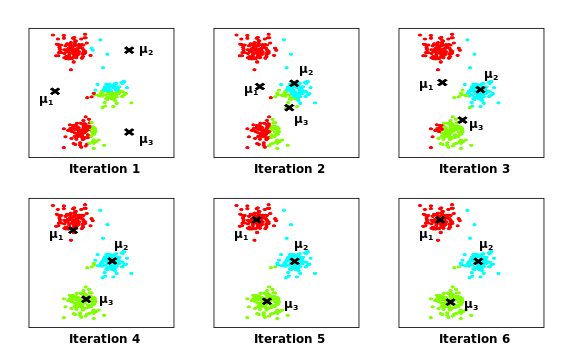
\includegraphics[width=\textwidth,height=3.9in]{prog.png}
\caption{Illustration of the $K$-means algorithm on a 2d data set with $K=3$.
Cluster assignment is shown by colour. The algorithm converges in 6 iterations}
\label{fig:kmeans-prog}
\end{figure*}

The algorithm then repeats the following two steps until convergence:
\begin{enumerate}
\item Assign each sample $x^{(i)}$ to the cluster represented by the centroid $\bs\mu_k$ that is closest to it.
\item Assign each cluster centroid $\bs\mu_k$ to the mean of all samples that currently belong to cluster $k$.
\end{enumerate}
The algorithm has converged once there are no more changes.
We have summarized the $K$-means algorithm in algorithm \ref{alg:kmeans}.

Figure \ref{fig:kmeans-prog} illustrates the algorithm with $K=3$ on a 2d data set consisting of 300 data points.
We chose a poor initialization for the cluster centroids so that we could show several iterations. 
With a better initialization, as suggested above, convergence would have been faster.



\subsection{Derivation and Convergence of $K$-Means}
\label{sect:kmeans-derivation}
In order to prove convergence of $K$-means, we define the \emph{distortion function} 
\begin{equation}
\label{eqn:distortion}
J(z^{(1)},\dots,z^{(N)},\bs\mu_1,\dots,\bs\mu_K) = \sum_{i=1}^N \sum_{k=1}^K \id\{z^{(i)}=k\}\,||\bs x^{(i)} - \bs \mu_k||^2
\end{equation}
The objective of $K$-Means clustering is equivalent to finding the parameters $z^{(i)} \in \{1,\dots,K\}$ and $\bs\mu_k\in\mathbb{R}^D$, for all $i$ and $k$, that minimize the distortion function $J$.

The $K$-means is obtained by applying the \emph{coordinate descent algorithm} to minimize the distortion function.
Coordinate descent is a simple optimization algorithm that can be used to find a local minimum of a multivariate function $F(\bs y)$.
It starts off by forming an initial guess $\bs y^{0}$ for the minimum $\bs y^*$. 
It then repeatedly cycles through each coordinate direction $y_j$ and minimizes $F$ along that direction.

In the case of the distortion function $J$, we only need to initialize the cluster centroids since the cluster assignments are independent of one another (the optimal value for $z^{(i)}$ tells us nothing about what $z^{(j)}$ should be).
We then minimize $J$ with respect to each $z^{(i)}$ keeping all other variables constant. 
If $K$ and $N$ are not too large, we can do this optimization by individually trying each value for $z^{(i)}$, i.e. by brute force.
The optimal value for $z^{(i)}$ is given by
\begin{equation}
\label{eqn:kmeans-E}
z^{(i)} = \argmin_k ||\bs x^{(i)} - \bs\mu_k||^2
\end{equation}
giving us the first inner loop of the $K$-means algorithm (lines 3-5 in algorithm \ref{alg:kmeans}).

Next, we minimize $J$ with respect to each cluster centroid $\bs\mu_k$ keeping all other variables constant.
We can do so by setting the gradient of $J$ with respect to $\bs\mu_k$ to zero:
\begin{equation}
\label{eqn:kmeans-M0}
\begin{split}
\nabla_{\bs\mu_k} J &= \nabla_{\bs\mu_k} \sum_{i=1}^N\id\{z^{(i)}=k\}(\bs x^{(i)}-\bs\mu_k)^T(\bs x^{(i)}-\bs\mu_k)\\
&= -2 \sum_{i=1}^N\id\{z^{(i)}=k\}(\bs x^{(i)}-\bs\mu_k) = 0\\
\end{split}
\end{equation}
Rearranging this equation gives us
\begin{equation}
\label{eqn:kmeans-M}
\Rightarrow \bs\mu_k = \frac{\sum_{i=1}^N\id\{z^{(i)} = k\}\,\bs x^{(i)}}{\sum_{i=1}^N\id\{z^{(i)}=k}
\end{equation}
This is the second inner loop of the algorithm (lines 6-8 in algorithm \ref{alg:kmeans}).
Furthermore, as already mentioned, (\ref{eqn:kmeans-M}) corresponds to setting $\bs \mu_k$ to the means of all samples $\bs x^{(i)}$ which currently assigned to cluster $k$.
\footnote{It is possible that $\sum_{i=1}^N\id\{z^{(i)}=k\} = 0$.
In other words, there is a possibility that a cluster becomes empty in the course of the algorithm.
If this happens, we can simply re-initialize the corresponding cluster centroid.
However, this may be an indication that we have set $K$ too large.}

One property of the coordinate descent algorithm is that each iteration is a (weak) improvement on the previous one.
This can be easily seen by noting that no update can make us worse off. 
So if the approximation to the solution at iteration $j$ is $\bs y^{(j)}$, then $F(\bs y^{(j)}) \geq F(\bs y^{(j+1)})$.
Hence, as long as the objective function is bounded below, the algorithm is guaranteed to converge to a local minimum.
Using the fact that $J \geq 0$, we have thus established convergence of the $K$-means algorithm.

Note, however, that we are only guaranteed to converge to a \emph{local} minimum.
Figure \ref{fog:kmeans-local} shows an example of a local optimum of the $K$-means algorithm applied to the same data set as in Figure \ref{fig:kmeans-prog}.

In two dimensions, we are able to visualize the data and might be able to identify a local solution simply by looking at the outcome. 
This is more difficult to do in higher dimensions.
In practice, this problem is dealt with by performing multiple runs of the entire $K$-Means algorithm.
We have to make sure that each run uses a different set of initial values for the the cluster centroids since, given an initialization, the $K$-means algorithm is completely deterministic.
We also need to record the final value of the distortion function $J$ after each run.
The overall output is then chosen to be the solution corresponding to the run for which the final value of $J$ was smallest.
Although this method does not guarantee convergence to the global optimum either, the resulting outcome is usually accepted to be at least ``good enough".

Convergence of the $K$-means algorithm was extensively studied by \cite{macqueen1967}.

\begin{figure}
\centering
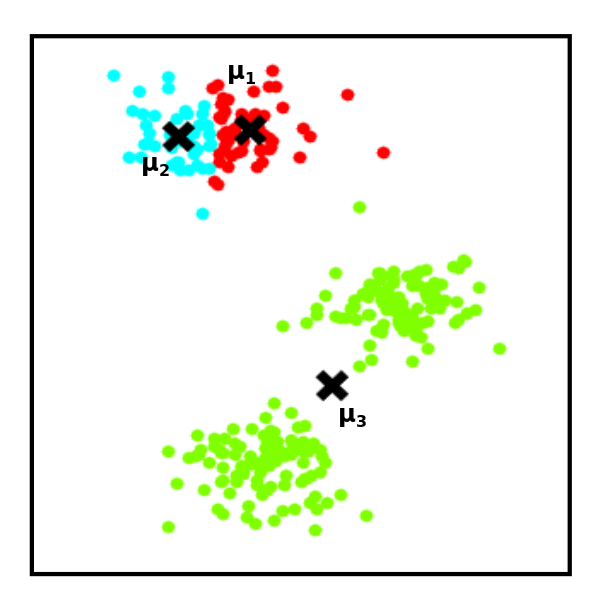
\includegraphics[width=3in]{local.png}
\caption{Local optimum of the K-Means algorithm applied to the data set from Figure \ref{fig:kmeans-prog} with $K=3$.}
\label{fig:kmeans-local}
\end{figure}



\subsection{Model selection for $K$-Means Clustering}
\label{sect:kmeans-ms}

\begin{figure*}
\centering
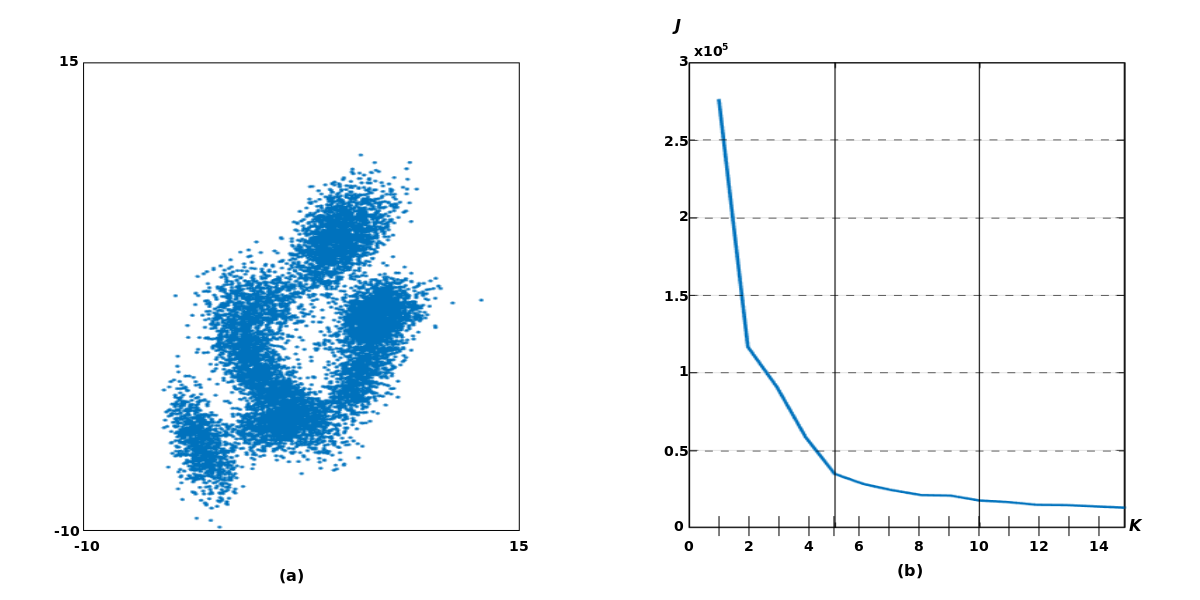
\includegraphics[width=\textwidth,height=3in]{elbow.png}
\caption{Illustration of the elbow method for selecting $K$ in $K$-means clustering. 
(a) Example 2d data set.
(b) We ran $K$-means on the data set in (a) for $1\leq K\leq 15$ and plotted the optimal value of the distortion function $J$ against $K$.}
\label{fig:kmeans-elbow}
\end{figure*}

The only user-set parameter in the $K$-means algorithm is the number of clusters.
Therefore, model selection for $K$-means amounts to selecting the optimal value for $K$.

The standard model selection tool for $K$-means clustering is the so-called ``elbow method" (also referred to as the ``kink method").
We run the $K$-Means algorithm for a range of different values of $K$, say for $1 \leq K \leq K_{max}$, where $K_{max}$ is some preset maximum value for $K$.
For each run, the optimal value of the distortion function, $J^*_K$, is saved.
If necessary, perform multiple random initializations for each $K$ to avoid poor local optima.
Finally, we plot $J_K^*$ against $K$.

In some cases, it is possible to identify a distinct ``kink" in the curve at some $K^*$ (i.e. the curve has a noticable ``elbow").
If that is the case, it would be a reasonable choice to set $K$ to the value at which the kink occurs.

The intuition is that, if there is some true number of clusters $K^*$, we would expect a steep slope in the elbow curve for $K < K^*$.
If $K < K^*$, we are putting several clusters into the same group. 
Splitting the group into its constituent clusters should have a large effect on the distortion function.

If $K > K^*$, we have broken individual clusters into smaller groups.
Thus, we would expect only a small reduction in the distortion compared to $K^*$.

We have illustrated the elbow method in Figure \ref{fig:kmeans-elbow}.
Note the disctinct ``kinks" at $K=3$ and $K=5$.
Looking at panel (a), either choice for $K$ could be a reasonable choice.

In practical applications, the optimal value for $K$ is often ambiguous.
In fact, a common behaviour of real-world data is that the number of clusters grows with the size of the data set.

Because of this, $K$ is usually chosen manually in practice.
In some applications, domain-specific knowledge may provide a reasonable value for $K$.



\subsection{Implementaion Details and Demonstration}
\label{sect:kmeans-code}
We have implemented the $K$-means algorithm in C++ using the external linear algebra library ``Armadillo" \cite{armadillo}.
Translating the pseudo-code in algorithm \ref{alg:kmeans} into C++ is straight-forward.
We only added two further features.
\begin{enumerate}
\item We put set a maximum value for the number of iterations in order to put a bound on the running time.
This is not strictly necessary since, as we saw in section \ref{sect:kmeans-derivation}, the algorithm is guaranteed to converge.
\item We run the algorithm multiple times, randomly re-initializing the centroids before each run.
We then save the output of the run for which $J$ was smallest.
As explained in section \ref{sect:kmeans-derivation}, this is done in order to mitigate the risk of getting a poor local optimum.
\end{enumerate}
A common demonstration of the $K$-means algorithm is image compression.
\begin{itemize}
\item Image compression
\item MNIST data
\end{itemize}



\subsection{Extensions and Generalizations of $K$-Means}
\label{sect:kmeans-concl}
In the introduction, we said that we would like data points inside the same cluster to be similar to each other and dissimilar to data points in other clusters.

The notion of similarity that we have been using in our discussion so far is based on squared Euclidean distance:
Two points $\bs x$ and $\bs x'$ are dissimilar if $||\bs x-\bs x'||^2$ is large.

It is possible to formulate the $K$-means algorithm using a general dissimilarity metric $V(\boldsymbol x, \boldsymbol x')$.
In that case, the distortion function takes the form
\begin{equation}
\label{eqn:kmedoid-distortion}
J(z^{(1)},\dots,z^{(N)},\bs \mu_1,\dots,\bs \mu_K) = \sum_{i=1}^N \sum_{k=1}^K \id\{z^{(i)}=k\}\,V(\bs x^{(i)}, \bs \mu_k)
\end{equation}
and the resulting algorithm is a generalization of $K$-means known as the \emph{$K$-medoids algorithm}.

Updating the cluster centroids in the $K$-medoids algorithm could be more complicated than in the $K$-means algorithm since the metric $V$ may not offer the same analytical convenience as the squared Euclidean metric.
One possible way of dealing with this problem is to restrict the cluster centroids $\bs\mu_k$ to be one of the data points $\bs x^{(i)}$ in cluster $k$.
This can be implemented as discrete search over the cluster.

Further extensions of the $K$-means algorithm are achieved by improving the cluster assignment step.
In its current form, we need to compute the squared Euclidean distance a total of $K$ times for each of the $N$ data points.
There have been proposals for speeding up this step (see \cite{Bishop} for a discussion and references).

In section \ref{sect:gmm}, we will discuss the Gaussian mixture model which can be regarded as a generalization of $K$-means to a probabilistic framework.

For more information on K-Means clustering, consult \cite{Bishop,Murphy}.






\section{Mixture Models and the EM Algorithm}
\label{sect:fmm}
The $K$-means algorithm provided us with a \emph{hard clustering} of the data.
This means that every data point $\bs x^{(i)}$ was assigned to a single cluster and we have no way of measuring the confidence of that assignment.
It could be that $\bs x^{(i)}$ ends up being very close to its cluster's centroid in which case the hard assignment is reasonable.
But it may also happen that $\bs x^{(i)}$ ends up being roughly midway between two centroids.
In that case, the hard assignment to the nearest centroid seems a lot less appropriate.

Ideally, we would like our cluster assignments to come with a measure of confidence, a so-called \emph{soft clustering}.
This section introduces a popular and simple approach to soft clustering.
We estimate the density of the data using a mixture model with $K$ components.
This will provide us with a posterior probabilities of each sample $\bs x^{(i)}$ belonging to the individual components of the model.
By viewing the components of the model, we end up with a soft clustering of our data into $K$ clusters.

We start off with a general desciption of finite mixture models in section \ref{sect:mixtures}.
We then discuss how to fit the parameters of the model using the \emph{EM algorithm}.

This section introduces mixture models and the EM algorithm in a general framework.
In section \label{sect:gmm}, we will discuss Gaussian mixtures, the most popular instance of finite mixture models.





\subsection{Mixture Models}
\label{sect:mixtures}
Suppose we have a data set $S = \{\bs x^{(1)},\dots,\bs x^{(N)}\}$ consisting of $N$ independent observations of a random variable $\bs X \in \mathbb{R}^D$.
We are interested in modelling the distribution of $\bs X$, i.e. we would like to use the data $S$ to estimate the probability density function $p(\bs x)$ of $\bs X$.

There are many ways of tackling this problem. 
The standard approach is to assume that $p(\bs x) = f(\bs x|\,\theta)$, i.e. that $p(\bs x)$ belongs to some family of distributions parametrized by $\theta$ and then use the data set $S$ to estimate $\theta$ with some inference method.
For example, a common technique is to assume $X$ is a Gaussian variable, such that 
\begin{equation}
f(\bs x |\,\theta) = \mathcal{N}(\bs x|\,\bs\mu,\bs \Sigma)
\end{equation}
and then use maximum likelihood estimation to infer the value of the parameter $\theta = (\bs\mu,\bs\Sigma)$.

The standard approach works well for simple data sets, but is somewhat limitted in more complex systems.
A simple way of extending this method is to assume that $p(\bs x)$ is composed of $K$ \emph{base distribution}.
Let $f_k(\bs x)$ denote the density function of the $k$th base distribution $F_K$.
The resulting density of $\bs X$ is then
\begin{equation}
\label{eqn:mixtures}
p(\bs x) = \sum_{k=1}^K \pi_k f_k(\bs x)
\end{equation}
We require $pi_k \geq 0$ for all $k$ and $\sum_{k=1}^K = 1$ in order for the density function to be well-defined.
Models of the form (\ref{eqn:mixtures}) are called \emph{mixture models}.

Mixture models are a special case of \emph{latent variable models}.
To see why, suppose we have discrete latent variable $Z$ taking values in $\{1,\dots,K\}$.
The distribution of $Z$ is fully specified by the quantities $\pi_1,dots,\pi_K$, where $\pi_k = \Pr(Z = k)$, and is referred to as the \emph{categorical distribution}, denoted $Z \sim \Cat(\pi_1, \dots,\pi_K)$.
We can express the probability mass function of $Z$ by
\begin{equation}
\label{eqn:cat}
\Cat(z|\,\bs\pi) = \prod_{k=1}^K \pi_k^{\id\{z=k\}}
\end{equation}
Note that, due their probabilistic nature, the parameters $\bs \pi = (\pi_1,\dots,\pi_K)$ must satisfy $\pi_k \geq 0$, $\sum_{k=1}^K \pi_k = 1$.

Out mixture models can then be built as follows:
\begin{equation}
\begin{split}
\label{eqn:mixture-lvm}
Z &\sim \Cat(\bs\pi)\\
\bs X |\,Z=k &\sim F_k
\end{split}
\end{equation}
The joint distribution of $\bs X$ and $Z$ is obtained from the product rule of probability:
\begin{equation}
\label{eqn:product-rule}
p(\bs x, z) = p(z)p(\bs x|\,z)
\end{equation}
Finally, to get the marginal ditribution of $\bs X$, we apply the sum rule of probability:
\begin{equation}
\label{eqn:sum-rule}
p(\bs x) = \sum_z p(\bs x, z)
\end{equation}

The resulting model is then derived as follows
\begin{equation}
\label{eqn:mixture-derivation}
\begin{split}
p(\bs x) &= \sum_z p(\bs x, z)\\
&= \sum_z p(z)p(\bs x|\,z)\\
&= \sum_{k=1}^K \Pr(Z=k) p(\bs x|\,Z=k)\\
&= \sum_{k=1}^K \pi_k f_k(\bs x)
\end{split}
\end{equation}
This is the same as the mixture model in (\ref{eqn:mixtures}).

Typically, the base distributions are chosen to belong to the same parametric family and differ only in the value of their parameter, so that $f_k(\bs x) = f(\bs x|\, \theta_k)$.
In that case, the mixture distribution is given by
\begin{equation}
\label{eqn:mixture-model}
p(\bs x|\,\bs\pi,\bs\theta) = \sum_{k=1}^K \pi_k f(\bs x|\,\theta_k)
\end{equation}
where we have made the dependence on the parameters $\bs\pi$ and $\bs\theta = (\theta_1,\dots,\theta_K)$ explicit.


\subsection{The EM algorithm}
\label{sect:EM}
Given our data set $S=\{\bs x^{(1)},\dots,\bs x^{(N)}\}$, how do we infer the parameters of our mixture model (\ref{eqn:mixture-model})?
The standard inference method in frequentist statistics is to find the parameter value that maximizes the likelihood of the data. 
So if our model for the joint distribution of $\bs X$ is $p(\bs x|\,\bs\theta)$, the likelihood of our data set $S$ is given by
\begin{equation}
\label{eqn:likelihood}
\mathcal{L}(\bs\theta) = \prod_{i=1}^N p(\bs x^{(i)}|\,\bs \theta)
\end{equation}
and we would like to find $\bs \theta$ that maximises $\mathcal{L}(\bs\theta)$.
This inference method is known as \emph{maximum likelihood estimation}. 

For simple models this problem can often be solved analytically.
Unfortunately, this is generally not the case for latent variable models and mixture models, in particular.

In this section, we will introduce the \emph{Expectation-Maximization} (EM) algorithm \cite{dempster1977}.
It is powerful variational technique that can be used to find a maximum likelihood solution in models with latent variables.

In a general latent variable framework, we have a model for $p(\bs x,z\,|\,\bs\theta)$, the joint distribution of the observed variable $\bs X$ and the latent variable $Z$ with parameter $\bs\theta$. 
The log likelihood of the data $S$ is 
\begin{equation}
\label{eqn:EMlikelihood}
\begin{split}
\ell(\bs\theta) &= \sum_{i=1}^N \log p(\bs x^{(i)}|\,\bs\theta)\\
&= \sum_{i=1}^N \log \left( \sum_{z^{(i)}} p(\bs x^{(i)},z^{(i)}|\,\bs\theta)\right)
\end{split}
\end{equation}
The sum inside the logarithm is what generally makes this optimization problem analytically intractable.
The expectation-maximization algorithm uses a simple iterative approach, often with closed-form updates at each step.
It alternated between two steps.
In the expectation (E) step, it forms a function that is a lower bound to $\ell(\bs\theta)$ and that is tight at the current value of $\bs\theta$.
In the maximization (M) step, it finds $\bs\theta$ that maximizes this lower bound.
This guarantees that we increase the value of $l(\theta)$ in each step until we find a local maximum.

In the following, we will derive the general form of the EM algorithm for maximizing the log likelihood function (\ref{eqn:EMlikelihood}).
We are treating $Z$ as a discrete latent variable, but the derivation is analogous for continuous $Z$ by simply exchanging the relevant sums with integrals.

We start by letting $Q_i(z^{(i)})$ be any probability function for $Z^{(i)}$. 
That means $Q_i(z^{(i)}) \geq 0$ and $\sum_{z^{(i)}} Q_i(z^{(i)}) = 1$. 
Our objective function can then be expressed as
\begin{equation}
\begin{split}
\ell(\bs\theta) &= \sum_{i=1}^N \log\left(\sum_{z^{(i)}} p(\bs x^{(i)},z^{(i)}\,|\,\bs\theta)\right)\\
&= \sum_{i=1}^N \log \left(\sum_{z^{(i)}} Q_i(z^{(i)}) \frac{p(\bs x^{(i)},z^{(i)}\,|\,\bs\theta)}{Q_i(z^{(i)})}\right)\\
&= \sum_{i=1}^N \log \mathbb{E}_{z^{(i)} \sim Q_i}\left[\frac{p(\bs x^{(i)},z^{(i)}\,|\,\bs\theta)}{Q_i(z^{(i)})}\right]\\
\end{split}
\end{equation}
where we used the definition of the expectation operator.

\begin{figure}
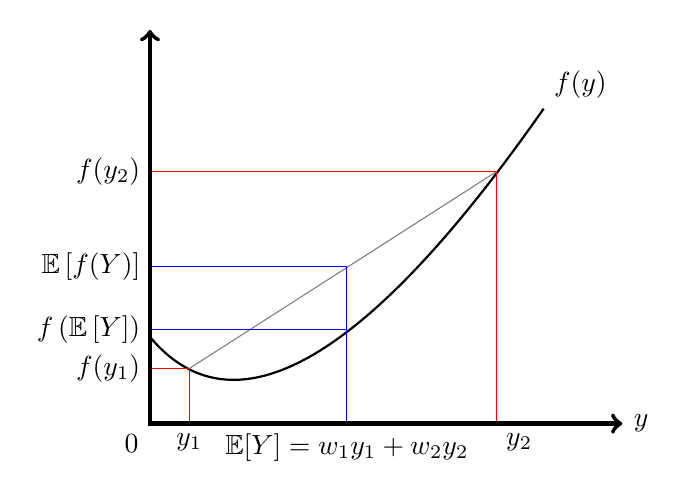
\begin{tikzpicture}
\draw [thick] (0,1.1) [out=310,in=235] to (5,4) node [above right] {$f(y)$};
\draw [gray] (0.5,0.7) -- (4.4,3.2);
\draw [thin, red] (0.5,0.7) -- (0.5,0) node [black,below] {$y_1$};
\draw [thin, red] (4.4,3.2) -- (4.4,0) node [black,below right] {$y_2$};
\draw [thin, red] (0.5,0.7) -- (0,0.7) node [black,left] {$f(y_1)$};
\draw [thin, red] (4.4,3.2) -- (0,3.2) node [black, left] {$f(y_2)$};
\draw [thin, blue] (2.5,2) -- (2.5,0) node [black, below] {$\mathbb{E}[Y]=w_1y_1+w_2y_2$};
\draw [thin, blue] (2.5,2) -- (0,2) node [black, left] {$\mathbb{E}\left[f(Y)\right]$};
\draw [thin, blue] (2.5,1.2) -- (0,1.2) node [black, left] {$f\left(\mathbb{E}\,[Y]\right)$};
\draw [ultra thick,<->] (0,5) -- (0,0) [below left] node{$0$} -- (6,0) node [right] {$y$};
\end{tikzpicture}
\caption{Illustration of Jensen's Inequality.
The random variable $Y$ can take two possible states $y_1$ and $y_2$ with probabilities $w_1$ and $w_2=1-w_1$ respectively.
It $Y$ had only one possible state, say $y_1$, so that $\Pr(Y=y_1)=1$, then $f\left(\mathbb{E}[Y]\right)$ and $\mathbb{E}\left[f(Y)\right]$ would coincide.
}
\label{fig:jensen}
\end{figure}

To proceed, we make use of \emph{Jensen's Inequality}:
Let $Y$ be a random variable and $f$ a convex function. Then
\begin{equation}
f\left(\mathbb{E}[Y]\right) \leq \mathbb{E}\left[f(Y)\right]
\label{eqn:jensen}
\end{equation}
Further, if $f$ is strictly convex, then the inequality is strict and we have
\begin{equation}
\mathbb{E}\left[f(Y)\right] = f\left(\mathbb{E}[Y]\right) \iff \Pr\left(Y = E[Y]\right) = 1
\label{eqn:jensentight}
\end{equation}
An illustration of Jensen's inequality is shown in Figure \ref{fig:jensen}.
If $f$ is concave, then the holds in inequality reverse since $(-f)$ is convex in that case. 

Applying Jensen's inequality to (\ref{eqn:EMlikelihood}) and using the fact that the log function is strictly concave gives us
\begin{equation}
\begin{split}
\ell(\bs\theta) &=  \sum_{i=1}^N \log \mathbb{E}_{z^{(i)} \sim Q_i}\left[\frac{p(\bs x^{(i)},z^{(i)}\,|\,\bs\theta)}{Q_i(z^{(i)})}\right]\\
&\geq \sum_{i=1}^N \mathbb{E}_{z^{(i)} \sim Q_i}\left[\log \frac{p(\bs x^{(i)},z^{(i)}\,|\,\bs\theta)}{Q_i(z^{(i)})}\right]\\ 
&= \sum_{i=1}^N \sum_{z^{(i)}} Q_i(z^{(i)}) \log \left(\frac{p(\bs x^{(i)},z^{(i)}\,|\,\bs\theta)}{Q_i(z^{(i)})}\right) := J(\bs\theta,\bs Q)
\end{split}
\end{equation}
where we used $\bs Q$ to denote $\{Q_1,\dots,Q_N\}$.

$J(\bs\theta,\bs Q)$ is a lower bound to the log likelihood function $\ell(\bs\theta)$ for \emph{any} valid choice of probability functions $\bs Q$.
What should our choice for the $Q_i$ be?

The EM algorithm makes the following choice.
Suppose we currently have an estimate of our parameters $\bs\theta^{\,(current)}$. 
In the E-step, the EM algorithm chooses $Q_i$ so that the lower bound is tight at $\bs\theta^{\,(current)}$, i.e. so that
\begin{equation}
J\left(\bs\theta^{\,(current)},\bs Q\right) = \ell\left(\bs\theta^{\,(current)}\right)
\end{equation}
Jensen's inequality tells us that this can be achieved by setting 
\begin{equation}
\frac{p(\bs x^{(i)},z^{(i)}\,|\,\bs \theta^{\,(current)})}{Q_i(z^{(i)})} = constant
\end{equation}
for all values of $z^{(i)}$.
This implies that
\begin{equation}
Q_i(z^{(i)}) \propto p(\bs x^{(i)},z^{(i)}\,|\,\bs\theta^{\,(current)})
\end{equation}
The constant of proportionality can be calculated by using the constraint that $\sum_{z^{(i)}} Q_i(z^{(i)}) = 1$.
Thus,
\begin{equation}
\label{eqn:EM-E}
\begin{split}
Q_i(z^{(i)}) &= \frac{p(\bs x^{(i)},z^{(i)}\,|\,\bs\theta^{\,(current)})}{\sum_{z^{(i)}}p(\bs x^{(i)},z^{(i)}\,|\,\bs\theta^{\,(current)})}\\
&= \frac{p(\bs x^{(i)},z^{(i)}\,|\,\bs\theta^{\,(current)})}{p(\bs x^{(i)}\,|\,\bs\theta^{\,(current)})}\\
&= p(z^{(i)}\,|\,\bs x^{(i)},\bs\theta^{\,(current)})
\end{split}
\end{equation}
where the second line follows from the sum rule of probability (\ref{eqn:sum-rule}) and the third line follows from the definition of conditional probabilities.
%This completes the E-Step of the EM algorithm.
Small digression: These quantities have an important interpretation in the context of soft clustering using mixture models.
They are the posterior distributions of the cluster assignments of our data are referred to as \emph{responsibilities}.
We say that $\Pr(z^{(i)} = k\,|\,\bs x^{(i)},\bs\theta)$ is the responsibility that cluster $k$ takes in explaining sample $\bs x^{(i)}$, and denote it $\gamma_k^{(i)}$.

Setting $Q_i(z^{(i)})$ completes the E-step of the EM algorithm.
In the M-Step, we update our parameters by finding $\bs\theta^{\,(new)}$ that maximizes this lower bound, keeping the $Q_i$ fixed.
In other words, we solve the following optimization problem
\begin{equation}
\label{eqn:EM-M}
\begin{split}
\bs\theta^{\,(new)} &= \argmax_{\bs\theta} J(\bs\theta,\ol{\bs Q}) \\
&= \argmax_{\bs\theta}\sum_{i=1}^N \sum_{z^{(i)}} \ol{Q_i}(z^{(i)}) \log \left( \frac{p(\bs x^{(i)},z^{(i)}\,|\,\bs\theta)}{\ol{Q_i}(z^{(i)})}\right) 
\end{split}
\end{equation}
where $\ol{Q_i}(z^{(i)}) = p(z^{(i)}\,|\,\bs x^{(i)},\bs\theta^{\,(current)})$.
\footnote{Thus, it is possible to interpret the EM algorithm as a particular instance of the coordinate ascent algorithm applied to the function $J(\bs\theta,\bs Q)$.}
This optimization problem is simpler than the direct optimization of the original log likelihood (\ref{eqn:EMlikelihood}).
In particular, it is possible to find a simple closed-form solution for a wide range of models, including the Gaussian mixture model.

We have summarized the general form of the EM algorithm in algorithm \ref{alg:EM}.

\begin{algorithm}
\caption{EM algorithm}
\label{alg:EM}
\begin{algorithmic}[1]
\State Initialize $\bs\theta^{\,(current)}$
\Statex\Repeat
\Statex $\qquad$ E-Step:
\For{$i = 1,\dots,N$}
\State Set $Q_i(z^{(i)}) = p(z^{(i)}\,|\,\bs x^{(i)},\bs\theta^{\,(current)})$
\EndFor
\Statex\Statex $\qquad$ M-Step:
\State $\bs\theta^{\,(new)} = \argmax_{\bs\theta}\sum_{i=1}^N \sum_{z^{(i)}} Q_i(z^{(i)}) \log \left( \frac{p(\bs x^{(i)},z^{(i)}\,|\,\bs\theta)}{Q_i(z^{(i)})}\right)$
\State Set $\theta^{\,(current)} = \theta^{\,(new)}$
\Until{Convergence}
\Statex\State\Return{  $\bs\theta^{\,(current)},z^{(1)}, \dots, z^{(N)}$}
\end{algorithmic}
\end{algorithm}




\section{The Gaussian Mixture Model}
\label{sect:gmm}
The Gaussian mixture model (GMM) (also known as mixtures of Gaussians) is the most widely used mixture model.
Before we explore its applications to clustering, let us first discuss the related problem of density estimation.
The goal of density estimation is to build the density $p(\boldsymbol x)$ of the random variable $\boldsymbol x \in \mathbb{R}^D$, given a set $\{\boldsymbol x^{(i)}\}_{i=1}^N$ of $N$ observations of $\boldsymbol x$.

Once we have formed the density $p(\boldsymbol x)$, we can apply the model to the problem of \emph{anomaly detection}.
Given a new observation $\boldsymbol x^{(N+1)}$, we flag it as an anomaly if $p(\boldsymbol x^{(N+1)}) < \epsilon$, where $\epsilon > 0$ is a pre-defined threshold.

The classical approach to density estimation is to assume $p(\boldsymbol x)$ belongs to some parametric family of distributions and to then infer the parameters from the data using tools such as \emph{maximum likelihood estimation}. 

\subsection{Modelling densities as mixtures of Gaussians}

What do we do if our data does not seem to come from any of the standard distributions (eg figure \ref{fig:gmm1}).

One approach is to do non-parametric density estimation. A more straight forward strategy is to use a mixture model.
In the GMM, we assume that the data was generated from $K$ distinct Gaussian \emph{base distributions}. 
We do not know which Gaussian generated which data points, so we introduce the discrete latent variable $z^{(i)} \in \{1,2,\dots,K\}$ that tells us which cluster sample $\boldsymbol x^{(i)}$ belongs to.

We assume that 
\begin{equation}
z \sim Discrete(\,\boldsymbol \pi)
\label{eqnzdistro}
\end{equation}
\begin{equation}
\boldsymbol x \,|\, z \sim \mathcal{N}(\,\boldsymbol{\mu_z}, \boldsymbol \Sigma_z)
\label{eqn:x|z-distro}
\end{equation}
This means
\begin{equation}
p(z) = \pi_z, \qquad \pi_k > 0 \, \forall k \in \{1,\dots,K\}, \sum_{k=1}^K \pi_k = 1 
\end{equation}
\begin{equation}
\begin{split}
p(\boldsymbol x\,|\,z) &= \mathcal{N}(\boldsymbol x\,|\, \boldsymbol \mu_z, \boldsymbol \Sigma_z) \\
&= \frac{1}{\sqrt{2\pi\,|\Sigma_z|}}\exp(-\frac{1}{2}(\boldsymbol x - \boldsymbol \mu_z)^T\boldsymbol \Sigma_z^{-1} (\boldsymbol x - \boldsymbol \mu_z))\\
\end{split}
\end{equation}

From the sum rule and product rule of probability, we have
\begin{equation}
\begin{split}
p(\boldsymbol x) &= \sum_z p(\boldsymbol x, z) \\
&= \sum_z p(z)p(\boldsymbol x \,|\, z)\\
&= \sum_{k=1}^K \pi_k \mathcal{N}(\boldsymbol x\,|\,\boldsymbol \mu_k, \boldsymbol \Sigma_k)
\label{eqn:gmmdensity}
\end{split}
\end{equation}

\subsection{The EM algorithm for the GMM}
Given a training set $S$, how to we fit the model parameters $\{\pi_k, \boldsymbol \mu_k, \boldsymbol \Sigma_k; k=1,\dots,K\}$?
	If the labels $z^{(i)}$ were observed, we could formulate the likelihood of the data \footnote{In this case the model is equivalent to the quadratic discriminant analysis model used for classification} 
\begin{equation}
\mathcal{L}(\pi_k, \boldsymbol \mu_k, \boldsymbol \Sigma_k) = \prod_{i=1}^N p(\boldsymbol x^{(i)},z^{(i)}\,|\,\pi_k, \boldsymbol \mu_k, \boldsymbol \Sigma_k)
\label{eqn:LDAlikelihood}
\end{equation}
Maximising the likelihood would yield the following solutions for $k = 1,\dots,K$:
\begin{equation}
\begin{split}
\label{eqn:LDAstats}
&\pi_k = \frac{\sum_{i=1}^N \mathbbm{1}\{z^{(i)} = k\}}{N}\\
&\mu_k = \frac{\sum_{i=1}^N \mathbbm{1}\{z^{(i)} = k\} \boldsymbol{x}^{(i)}}{\sum_{i=1}^N \mathbbm{1}\{z^{(i)} = k\}}\\
&\Sigma_k = \frac{\sum_{i=1}^N \mathbbm{1}\{z^{(i)} = k\} (\boldsymbol{x}^{(i)} - \boldsymbol \mu_k)(\boldsymbol{x}^{(i)} - \boldsymbol \mu_k)^T}{\sum_{i=1}^N \mathbbm{1}\{z^{(i)} = k\}}\\
\end{split}
\end{equation}
(See the appendix for a derivation.)

In the unsupervised setting, we do not observe the values of $z^{(i)}$. 
Thus, the likelihood of our data now takes the form
\begin{equation}
	\mathcal{L}(\boldsymbol \pi, \boldsymbol \mu, \boldsymbol \Sigma) = \prod_{i=1}^N p(\boldsymbol x^{(i)}\,|\,\boldsymbol \pi, \boldsymbol \mu, \boldsymbol \Sigma)\\
\label{eqn:gmmLikelihood}
\end{equation}
Taking logs on both side and using equation \ref{eqn:gmmdensity}, we can formulate our objective function as
\begin{equation}
\begin{split}
\log\mathcal{L}(\boldsymbol \pi, \boldsymbol \mu, \boldsymbol \Sigma) &= \sum_{i=1}^N \log p(\boldsymbol x^{(i)}\,|\,\boldsymbol \pi \boldsymbol \mu, \boldsymbol \Sigma)\\
&= \sum_{i=1}^N \log \left(\sum_{k=1}^K \pi_k \mathcal{N}(\boldsymbol x^{(i)}\,|\, \boldsymbol \mu_k, \boldsymbol \Sigma_k)\right)\\
\end{split}
\label{eqn:gmmlogLikelihood}
\end{equation}

Maximising this objective function directly is problematic due to summation inside the logarithm term and there is, in fact, no known closed form solution.
Instead we use an iterative scheme in which we first formulate a ``guess" for the $z^{(i)}$ given our current parameter values and then find the optimal model parameters given our guess. 

Formally, we build the \emph{responsibility} that cluster $k$ takes for explaning sample $\boldsymbol x^{(i)}$, denoted $\gamma_k^{(i)}$.
This is defined to be the posterior probabibility that $z^{(i)} = k$:
\begin{equation}
\label{eqn:gmmresponsibility}
\begin{split}
y_k^{(i)} &= p(z^{(i)}=k\,|\,\boldsymbol x^{(i)}; \boldsymbol \pi, \boldsymbol \mu, \boldsymbol \Sigma)\\
	&= \frac{p(z^{(i)}=k;\boldsymbol \pi)p(\boldsymbol x^{(i)}\,|\,z^{(i)}=k;\boldsymbol \mu, \boldsymbol \Sigma)}
	{\sum_{j=1}^K p(z^{(i)}=j;\boldsymbol \pi)p(\boldsymbol x^{(i)}\,|\,z^{(i)}=j;\boldsymbol \mu, \boldsymbol \Sigma)}\\
	&= \frac{\pi_k\mathcal{N}(\boldsymbol x^{(i)}\,|\,\boldsymbol \mu_k, \boldsymbol \Sigma_k)}
	{\sum_{j=1}^K \pi_j\mathcal{N}(\boldsymbol x^{(i)}\,|\,\boldsymbol \mu_j, \boldsymbol \Sigma_j)}
\end{split}
\end{equation}

Once we have calculated the responsibilities, we can use them to update our model parameters.
\begin{equation}
\label{eqn:gmmstats}
\begin{split}
\pi_k &= \frac{\sum_{i=1}^N \gamma_k^{(i)}}{N}\\
\boldsymbol \mu_k &= \frac{\sum_{i=1}^N \gamma_k^{(i)} \boldsymbol x^{(i)}}{\sum_{i=1}^N \gamma_k^{(i)}}\\
\boldsymbol \Sigma_k &= \frac{\sum_{i=1}^N \gamma_k^{(i)}(\boldsymbol x^{(i)} - \boldsymbol \mu_k)(\boldsymbol x^{(i)} - \boldsymbol \mu_k)^T}{\sum_{i=1}^N \gamma_k^{(i)}}\\
\end{split}
\end{equation}
Note that we use the new value of $\boldsymbol \mu_k$ to calculate $\boldsymbol \Sigma_k$ in equation \ref{eqn:gmmstats}.
We iterate these two steps until convergence.
The typical convergence criterion is that changes in the loglikelihood are below some threshold.

Note the similarity with equation \ref{eqn:LDAstats}.
We have essentially replaced the indicators with \emph{soft weights} $\gamma_k^{(i)}$.
In the limit in which we observe $z^{(i)}$, we put all the probability mass on the observed value of $z^{(i)}$ and obtain $\gamma_k^{(i)} = \mathbbm{1}\{z^{(i)} = k\}$.

The algorithm above is a particular instance of the \emph{Expectation-Maximization (EM)} algorithm.
Equation \ref{eqn:gmmresponsibility} corresponds to the \emph{expectation step (E-step)} and equation \ref{eqn:gmmstats} corresponds to the \emph{maximization step (M-Step)} of the EM algorithm.
We will discuss the EM algorithm in more detail in the next section and also derive equations \ref{eqn:gmmresponsibility} and \ref{eqn:gmmstats}.
The pseudo-code for fitting the model parameters for the GMM can be found in algorithm \ref{alg:gmm}.

\begin{algorithm}
\caption{EM algorithm for GMM}
\label{alg:gmm}
\begin{algorithmic}[1]
\Procedure{EM for GMM}{$\boldsymbol X,K$}
\State{Randomly initialize $(\pi_k, \boldsymbol \mu_k, \boldsymbol \Sigma_k)$ for $k=1,\dots,K$}
\Repeat
\For{$i = 1:N$}\Comment{E-Step}
\State{$\gamma_k^{(i)} = \frac{\pi_k\mathcal{N}(\boldsymbol x^{(i)}\,|\,\boldsymbol \mu_k, \boldsymbol \Sigma_k)}
	{\sum_{j=1}^K \pi_j\mathcal{N}(\boldsymbol x^{(i)}\,|\,\boldsymbol \mu_j, \boldsymbol \Sigma_j)}$}
\EndFor
\For{$k = 1:K$}\Comment{M-Step}
\State{$\pi_k = \frac{\sum_{i=1}^N \gamma_k^{(i)}}{N}$}
\State{$\boldsymbol \mu_k = \frac{\sum_{i=1}^N \gamma_k^{(i)} \boldsymbol x^{(i)}}{\sum_{i=1}^N \gamma_k^{(i)}}$}
\State{$\boldsymbol \Sigma_k = \frac{\sum_{i=1}^N \gamma_k^{(i)}(\boldsymbol x^{(i)} - \boldsymbol \mu_k)(\boldsymbol x^{(i)} - \boldsymbol \mu_k)^T}{\sum_{i=1}^N \gamma_k^{(i)}}$}
\EndFor
\Until{Convergence}
\EndProcedure \\
	\Return{$\{(\gamma^{(1)}_k, \dots, \gamma^{(N)}_k, \pi_k, \boldsymbol \mu_k, \boldsymbol \Sigma_k), \quad k = 1,\dots,K\}$}
\end{algorithmic}
\end{algorithm}




In the Gaussian mixture model, for the E-step we have
\begin{equation}
\label{eqn:gmmE}
\begin{split}
Q_i(z^{(i)} = k) &= p(z^{(i)} = k\,|\,\boldsymbol x^{(i)}; \boldsymbol \pi, \boldsymbol \mu, \boldsymbol \Sigma)\\
&= p(z^{(i)}=k\,|\,\boldsymbol x^{(i)}; \boldsymbol \pi, \boldsymbol \mu, \boldsymbol \Sigma)\\
&= \frac{p(z^{(i)}=k;\boldsymbol \pi)p(\boldsymbol x^{(i)}\,|\,z^{(i)}=k;\boldsymbol \mu, \boldsymbol \Sigma)}
{\sum_{j=1}^K p(z^{(i)}=j;\boldsymbol \pi)p(\boldsymbol x^{(i)}\,|\,z^{(i)}=j;\boldsymbol \mu, \boldsymbol \Sigma)}\\
&= \frac{\pi_k\mathcal{N}(\boldsymbol x^{(i)}\,|\,\boldsymbol \mu_k, \boldsymbol \Sigma_k)}
{\sum_{j=1}^K \pi_j\mathcal{N}(\boldsymbol x^{(i)}\,|\,\boldsymbol \mu_j, \boldsymbol \Sigma_j)} = \gamma_k^{(i)}
\end{split}
\end{equation}

While in the M-Step we want to find $\pi_k$, $\boldsymbol \mu_k$ and $\boldsymbol \Sigma_k$ that maximize
\begin{equation}
\label{eqn:gmmM1}
\begin{split}
J(\boldsymbol \pi, \boldsymbol \mu, \boldsymbol \Sigma, \boldsymbol \gamma) &= \sum_{i=1}^N\sum_{z^{(i)}} Q_i(z^{(i)}) \log \frac{p(\boldsymbol x^{(i)},z^{(i)};\boldsymbol \pi, \boldsymbol \mu, \boldsymbol \Sigma)}{Q_i(z^{(i)})}\\
&= \sum_{i=1}^N \sum_{k=1}^K \gamma_k^{(i)} \log \frac{\pi_j \mathcal{N}(\boldsymbol x^{(i)} \,|\, \boldsymbol \mu_k, \boldsymbol \Sigma_k)}{\gamma_k^{(i)}}\\
\end{split}
\end{equation}
Setting the derivative with respect to $\boldsymbol \mu_k$ equal to zero gives
\begin{equation}
\begin{split}
\label{eqn:gmmMu}
\nabla_{\boldsymbol \mu_k} J &= \sum_{i=1}^N -\frac{1}{2}\gamma_k^{(i)} \nabla_{\boldsymbol \mu_k} (\boldsymbol x^{(i)} - \boldsymbol \mu_k)^T \boldsymbol \Sigma^{-1}(\boldsymbol x^{(i)} - \boldsymbol \mu_k)\\
&= \sum_{i=1}^N -\frac{1}{2}\gamma_k^{(i)}(\boldsymbol \Sigma_k^{-1} + \boldsymbol \Sigma_k^{-T})(\boldsymbol \mu_k - \boldsymbol x^{(i)})\\
&= \sum_{i=1}^N\gamma_k^{(i)} \boldsymbol \Sigma^{-1} (\boldsymbol x^{(i)} - \boldsymbol \mu_k) = 0\\
\Rightarrow \boldsymbol \mu_k &= \frac{\sum_{i=1}^N\gamma_k^{(i)} \boldsymbol x^{(i)}}{\sum_{i=1}^N \gamma_k^{(i)}}
\end{split}
\end{equation}
To find the optimal $\boldsymbol \Sigma_k$, we note that this equivalent to finding $\boldsymbol \Sigma_k^{-1}$ that maximizes $J$:
\begin{equation}
\label{eqn:gmmSigma}
\begin{split}
\nabla_{\boldsymbol \Sigma_k^{-1}} J &= \sum_{i=1}^N \gamma_k^{(i)}(\frac{1}{2}\nabla_{\boldsymbol \Sigma_k^{-1}}(\log |\boldsymbol \Sigma_k^{-1}| - (\boldsymbol x^{(i)} - \boldsymbol \mu_k)^T \boldsymbol \Sigma_k^{-1}(\boldsymbol x^{(i)} - \boldsymbol \mu_k))\\
&= \sum_{i=1}^N \gamma_k^{(i)} \frac{1}{2}(\boldsymbol \Sigma_k - (\boldsymbol x^{(i)} - \boldsymbol \mu_k)(\boldsymbol x^{(i)} - \boldsymbol \mu_k)^T) = 0\\
\Rightarrow \boldsymbol \Sigma_k &= \frac{\sum_{i=1}^N \gamma_k^{(i)}(\boldsymbol x^{(i)} - \boldsymbol \mu_k)(\boldsymbol x^{(i)} - \boldsymbol \mu_k)^T}{\sum_{i=1}^N \gamma_k^{(i)}}
\end{split}
\end{equation}
The mixing coefficients $\boldsymbol \pi$ must satisfy the constraint $\sum_{k=1}^K \pi_k = 1$.
We use the method of Lagrange multipliers to perform the constrained optimization.
Let $\lambda > 0$ denote the Lagrange multiplier.
To find the optimal coefficients $\pi_k$, we set the derivative of $(J(\boldsymbol \pi, \boldsymbol \mu, \boldsymbol \Sigma, \boldsymbol \gamma) + \lambda(1-\sum_{k=1}^K \pi_k))$ with respect to $\pi_k$ to zero.
\begin{equation}
\label{eqn:gmmPi1}
\begin{split}
\frac{\partial}{\partial \pi_k}(J + \lambda(1 - \sum_{k=1}^K \pi_k)) &= \sum_{i=1}^N\gamma_k^{(i)} \frac{\partial}{\partial \pi_k} \log \pi_k - \lambda\\
&= \sum_{i=1}^N \frac{\gamma_k^{(i)}}{\pi_k} - \lambda = 0\\
\Rightarrow \pi_k = \frac{\sum_{i=1}^N\gamma_k^{(i)}}{\lambda}
\end{split}
\end{equation}
Taking the sum over $k$ on both sides gives
\begin{equation}
\label{eqn:gmmPi2}
\begin{split}
1 &= \frac{\sum_{i=1}^N \sum_{k=1}^K \gamma_k^{(i)}}{\lambda}\\
\Rightarrow \lambda &= \sum_{i=1}^N \sum_{k=1}^K \gamma_k^{(i)}\\
&= \sum_{i=1}^N 1 = N
\end{split}
\end{equation}
Since $\sum_{k=1}^K \gamma_k^{(i)} = \sum_{k=1}^K p(z^{(i)} = k\,|\,\boldsymbol x^{(i)}) = 1$.
Thus,
\begin{equation}
\pi_k = \frac{\sum_{i=1}^N \gamma_k^{(i)}}{N}.
\label{eqn:gmmPi3}
\end{equation}

\subsection{Model Selection in the Gaussian mixture model}
It is possible for the EM algorithm to get stuck in local optima.
The approach of dealing with this problem is analogous to the one used in the K-Means algorithm:
We perform multiple runs of the EM algorithm with different random initializations of the GMM parameters. We then pick the result for which the log likelihood was greatest.

In order to choose $K$, we may again employ the ``elbow method'', by plotting the negative log likelihood against $K$.
Another popular approach is the use information theoretic model selection criteria such as the \emph{Akaike Information Criterion (AIC)}, the \emph{Bayesian Information Criterion (BIC)} or the \emph{Kullbeck-Leibler Information Criterion (KLIC)}.
It is also possible to embed the GMM in a Bayesian framework by putting prior probabilities on our model parameters.
For instance, we could put a Gaussian-Inverse-Wishart prior on the cluster means and covariances and a Dirichlet prior on the mixing coefficients.
These priors are conjugate to our likelihood function and thus lead to fast computation of the posterior probabilities of the parameters. \emph{(CHECK THIS)}.
\emph{COMMENT: how is this used for model selection?}

\subsection{KMeans as limit of GMM}
We can derive the K-Means algorithm as a special case of the EM algorithm for the Gaussian Mixture Model.
Let is fix $\pi_k = 1/K$ and $\boldsymbol \Sigma_k = \sigma^2 \boldsymbol I_D$ for all values of $k$.
Further, let us approximate the responsibilities by delta functions
\begin{equation}
\label{eqn:gmmdelta}
\gamma_k^{(i)} = \mathbbm{1}\{z^{(i)} = k^*\}
\end{equation}
where
\begin{equation}
k^* = \argmax_k p(z^{(i)} = k\,|\,\boldsymbol x^{(i)},\boldsymbol \pi, \boldsymbol \mu, \boldsymbol \Sigma)
\end{equation}
is the MAP estimate of $z^{(i)}$.
Due to the spherical covariance matrix, $k^*$ will be simply equal to the identity of the currently closest cluster centroid to $\boldsymbol x^{(i)}$. This completes the E-step.

In the M-Step, we only need to update the cluster means $\boldsymbol \mu_k$.
Using our approximations for $\gamma_k^{(i)}$, the GMM update formula for $\boldsymbol \mu_k$ reduces to the one we used in the K-Means algorithm, i.e. the empirical mean of all data points currently assigned to cluster $k$.

For more info, see \cite{Bishop} and \cite{Murphy}.

\section{Extensions and Further Work}
Conclusion.

\section*{Acknowledgements}
Here I acknowledge the assistance of my supervisor, my industrial sponsor,
and the effects of caffine on my ability to produce this report on time.

%% The Appendices part is started with the command \appendix;
%% appendix sections are then done as normal sections
\appendix


%% References
%%
%% Following citation commands can be used in the body text:
%% Usage of \cite is as follows:
%%   \cite{key}         ==>>  [#]
%%   \cite[chap. 2]{key} ==>> [#, chap. 2]
%%

%% References with bibTeX database:
\section*{Bibliography}
\bibliographystyle{elsarticle-num}
\bibliography{references.bib}

%% Authors are advised to submit their bibtex database files. They are
%% requested to list a bibtex style file in the manuscript if they do
%% not want to use elsarticle-num.bst.

%% References without bibTeX database:

% \begin{thebibliography}{00}

%% \bibitem must have the following form:
%%   \bibitem{key}...
%%

% \bibitem{}

% \end{thebibliography}


\end{document}

%%
%% End of file `mini.tex'.